% \addcontentsline{toc}{part}{Part II}
\chapter{\label{cha:algorithm} Test Program-Based Fuzzing for the Kotlin Compiler}

This chapter details the foundational techniques, abstractions,
and trade-offs that our novel approach employs to generate syntactically
valid and semantically meaningful Kotlin code.
\section{\label{sec:approachoverview}Approach Overview}

We design our approach along three main pillars, broadly depicted in \Cref{fig:approach}.
The first two pillars tackle the fuzzer's internal connection to Kotlin
through semantics and syntax.
The third coalesces the interfaces provided by the first two
into a powerful representation which allows the integration of complex
heuristic approaches into the fuzzing process.

\Cref{sec:context} addresses the first core component of the fuzzer,
which  handles the semantics of Kotlin.
This module contains representations for a wide range
of Kotlin code constructs, a detailed type hierarchy, and
adaptable constraints that aid with code generation at runtime.
In addition, this \textit{context} component is equipped with
an extraction procedure that allows users to customize
the semantic environment in which the fuzzer operates.

\Cref{sec:syntax} discusses the syntax handling module of the fuzzer.
This component operates on a specification of the Kotlin \gls{CFG},
which it transforms into a truncated version.
The transformation additionally equips the grammar with
operations that integrate with its context-handling counterpart,
in turn enhancing versatility and configurability of the fuzzer.

Sections \ref{sec:repr} and \ref{sec:heuristics} outline the final pillar
of our approach.
The former establishes a hierarchical structure that aligns code
within generated files with its local dependencies, enabling
powerful mutation operators.
The latter develops this structure into three classes of
search algorithms.
Finally, a fourth auxiliary configuration component
augments the three main pillars and allows users
to select from the many techniques established in this chapter.

% Define block styles
\tikzset{%
  materia/.style={draw, fill=gray!20, text width=6.0em, text centered, minimum height=1.5em,drop shadow},
  etape/.style={materia, text width=8em, minimum width=10em, minimum height=3em, rounded corners, drop shadow},
  texto/.style={above, text width=6em, text centered},
  linepart/.style={draw, thick, color=black!50, -LaTeX, dashed},
  line/.style={draw, thick, color=black, -LaTeX},
  ur/.style={draw, text centered, minimum height=0.01em},
  back group/.style={fill=white,rounded corners, draw=black, dashed, inner xsep=15pt, inner ysep=10pt},
}

\newcommand{\etape}[2]{node (p#1) [etape] {#2}}

\newcommand{\transreceptor}[3]{%
  \path [linepart] (#1.east) -- node [above] {\scriptsize #2} (#3);}

\begin{figure}
    % \centering
\begin{tikzpicture}

  % Draw diagram elements
  \path \etape{1}{Kotlin Files};
  \path (p1.east)+(3.5,0.0) \etape{2}{Grammar Spec};
  \path (p2.east)+(3.5,0.0) \etape{3}{Config Spec};
  
  \path (p1.south)+(0.0,-1.5) \etape{4}{Context};
  \path (p2.south)+(0.0,-1.5) \etape{5}{Extended CFG};
  \path (p3.south)+(0.0,-1.5) \etape{6}{Configuration};

  \path (p5.south)+(0.0,-1.5) \etape{7}{Search Algorithm};
  \path (p7.south)+(0.0,-1.5) \etape{8}{Generated Code};
  \path (p8.east)+(3.5,0.0) \etape{9}{\texttt{K1} Compiler};
  \path (p8.west)+(-3.5,0.0) \etape{10}{\texttt{K2} Compiler};

  \path (p1.north)+(0.0,0.65) node (p11) {\Cref{sec:context}};
  \path (p2.north)+(0.0,0.65) node (p11) {\Cref{sec:syntax}};
  \path (p3.north)+(0.0,0.65) node (p11) {\Cref{sec:configuration}};
  % Draw arrows between elements
  \path [line] (p1.south) -- node [above] {} (p4);
  \path [line] (p3.south) -- node [above] {} (p6);
  \path [line] (p2.south) -- node [above] {} (p5);
  \path [line] (p5.south) -- node [above] {} (p7);
  \path [line] (p4.south) -- node [left] {} (p7);
  \path [line] (p6.south) -- node [right] {} (p7);
  \path [line] (p7.south) -- node [above] {} (p8);
  \path [line] (p9.west) -- node [left] {} (p8);
  \path [line] (p10.east) -- node [right] {} (p8);

  \path (p7.east)+(+3.0,0) node (ur1)[ur] {};
  \transreceptor{p7}{Sections \ref{sec:repr}, \ref{sec:heuristics}}{ur1};
   
  \begin{scope}[on background layer]
    \node (bk1) [back group] [fit=(p1) (p4)] {};
    \node (bk2) [back group] [fit=(p2) (p5)] {};
    \node (bk3) [back group] [fit=(p3) (p6)] {};\
    \node (bk4) [back group] [fit=(p8) (p9) (p10)] {};
  \end{scope}
\end{tikzpicture}

    \caption{Conceptual layout of the approach.}
    \label{fig:approach}
\end{figure}
\section{\label{sec:context}Semantic Interface}

Kotlin is a rich programming language, that conjoins various
paradigms, each building upon numerous layers of
theoretical abstractions.
These abstractions collectively govern the semantics
of the language, and implicitly determine the validity of programs.
We jointly represent the core concepts that compose the Kotlin
semantics, as well as the constraints that underlie their behavior,
under an construct concept called the fuzzer's \textit{context}.

The context contains both adaptive, program-specific details (such as scopes and
visible identifiers), and universally applicable statues (such as type hierarchies).
The information encapsulated in the context drives the generative
process, similarly to \textsc{YARPGen} \cite{manes2019art}.
However, unlike \textsc{YARPGen}, we endow our representation of the context
with an extraction feature that allows the parsing of arbitrary
Kotlin code to serve as the basis of further generation. 
The remainder of this section describes three key features of the context.
\Cref{subsec:type-hierarchy} first addresses the type hierarchy
representation.
\Cref{subsec:callables} describes the internal representation
of language structures.
Finally, \Cref{subsec:context-extraction} lays out
the automated context extraction process.

\newacronym{DAG}{DAG} {Directed Acyclic Graph}

\subsection{\label{subsec:type-hierarchy}Type Hierarchy Representation}

Kotlin is a strongly-typed language, with well-formed semantics
that are crucial for generating valid code snippets.
We represent these the Kotlin type system using a labeled \Gls{DAG} data structure.
Formally, a \Gls{DAG} $G$ is a tuple $\langle V, E \rangle$ composed
of a set of vertices $V$ and a function $E : (V \times V) \to L^{+}$ that
each link pairs of vertices in $V$ through a composite transition from a domain $L$.

The set $V$ comprises all the accessible \textit{classifier} (classes and interfaces) types
(i.e., (abstract) classes, interfaces) in the environment.
The function $E$ maps each pair of vertices $\langle u, v \rangle$ with $u, v \in V$
to a label $l \in L = \{ \emptyset, >, \epsilon \} \cup V$, where the label signifies
the inheritance relation between the two types.
A $\emptyset$ transition signals that there is no direct relation between types, while
a $>$ transitions symbolizes that $v$ is a direct and unparameterized subtype of $u$.
To accommodate the semantics of parameterized types, we enrich the label set $L$
with all types belonging to $V$, as well as an additional symbol $\epsilon$.
A label belonging to $V$ signifies that one of the parameterized types of $u$
explicitly belongs to a type hierarchy, while the $\epsilon$ transition represents
the inheritance of a symbolic type.

\begin{figure}
    \footnotesize
    \centering
	\begin{tikzpicture}
	\begin{scope}[every node/.style={circle,thick,draw} ]
		\node[minimum size=30pt] (D) at (5,4) {\texttt{Any}};
    		\node[minimum size=30pt] (A) at (0,4) {\texttt{Number}};
    		\node[minimum size=30pt] (B) at (5,1) {\tiny\texttt{Comparable$<$E$>$}};
    		\node[minimum size=30pt] (C) at (0,1) {\texttt{Double}};
    		\node[minimum size=30pt] (E) at (10,4) {\scriptsize\texttt{Iterable$<$E$>$}};
    		\node[minimum size=30pt] (F) at (10,1) {\tiny\texttt{Collection$<$E$>$}};
	\end{scope}
	\begin{scope}[>={Stealth[black]},
              every node/.style={fill=white,circle},
              every edge/.style={draw=black,very thick}]
    		\path [->] (B) edge node {$\texttt{Double}$} (C);
    		\path [->] (A) edge node {$>$} (C);
    		\path [->] (D) edge node {$>$} (A);
	    	\path [->] (D) edge node {$>$} (B);
    		\path [->] (D) edge node {$>$} (E);
    		\path [->] (E) edge node {$\epsilon$} (F);
%    \path [->] (B) edge[bend right=60] node {$1$} (E); 
	\end{scope}
	\end{tikzpicture}
    \caption{A sample of the type hierarchy representation using standard Kotlin types.}
    \label{fig:type-hierarchy}
\end{figure}

\Cref{fig:type-hierarchy} depicts the \Gls{DAG} representation
a small subset of built-in and standard Kotlin types,
with $\emptyset$ transitions left out.
Within this hierarchy, the \texttt{Number}, \texttt{Comparable$<$E$>$}, 
and \texttt{Iterable$<$E$>$} types all directly inherit from the \texttt{Any} node, 
which is the root of the type hierarchy.
The \texttt{Number} and \texttt{Comparable$<$E$>$} have a common immediate descendant in the 
\texttt{Double} type, though their transitions differ.
The transition between \texttt{Comparable$<$E$>$} and \texttt{Double} itself
contains the annotation \texttt{Double}, an exact type referring to a node in the graph
that is required to complete the inheritance.
The $\epsilon$ label on the edge between \texttt{Iterable$<$E$>$} and \texttt{Collection$<$E$>$}
denotes that \texttt{E} is a symbolic type, and that a link between the two parameterized types
must be consistent.
The meaning of consistency is intricate,
as parameterized types in Kotlin may contain bounds
that further limit the domain of valid parameter types.
To integrate this constraint, bound information is additionally
stored in edge labels.

This representation of types offers several key advantages within the scope of the fuzzer.
First, a graph representation is flexible in that new types can easily be added, removed, or changed
during fuzzing.
This flexibility also enables automating the construction of a type hierarchy
from pre-written Kotlin files, which in turn allows for near-endless customization of the fuzzing space.
Second, a \Gls{DAG} topology enables the encoding of strict semantic constraints into
graph-centric problems.
This applies to simple inheritance semantics
(i.e., subclasses may be used wherever a superclass is expected),
but can also generalize to Kotlin-specific traits,
such as requiring children of the \texttt{Iterable$<$E$>$}
node whenever a \texttt{for} loop occurs.
Finally, the \Gls{DAG} greatly prunes the search space of semantically valid solutions, as simple graph walking
algorithms suffice to solve problems related to sound parameterized type inference, a common problem
when fuzzing the Kotlin standard library.

\subsection{\label{subsec:callables}Callable Representation}
In addition to a type hierarchy, the fuzzer uses knowledge to which \textit{callables}
it can act upon.
We use the term callable in a similar fashion to \citet{stepanov2021type}.
The collection of callables in the context encompasses
the set of functions, methods, constructors, variables, constants, and predefined primitive values
available to the fuzzer.
We model each callable as a 5-tuple $\langle N, O, P, I, R \rangle$ that builds on top of the
type hierarchy.
Let $N$ the name of the callable, $O$ the type of the callable's \textit{owner} class,
$P$ a list of (symbolic) parameterized types specific to the callable,
$I$ a list of input types that the callable requires,
and $R$ the return (or output type) of the callable.
This representation draws inspiration from lambda calculus and aims to provide a uniform representation
for all callables that Kotlin can represent.

\lstset{
  basicstyle=\footnotesize, frame=tb,
  xleftmargin=.2\textwidth, xrightmargin=.2\textwidth,
  numbers=left, stepnumber=1,
}

\begin{figure}
\begin{lstlisting}[language=Kotlin]
class Foo <E>(bar: String, baz: E) {
    val fooProp1: String = bar
    var fooProp2: E = baz
    fun <P> fooFunc(parameter: P) : E {
        return fooProp2
    }
}
\end{lstlisting}
\caption{Simple Kotlin snippet.}
\label{fig:callables}
\end{figure}

To help build intuition on the applicability of this representation,
consider the snippet depicted in \Cref{fig:callables}.
Though simple, the \texttt{Foo} class contains several representationally
challenging constructs that help illustrate the capability of the callable construct.
First, the \texttt{Foo$<$E$>$} type itself belongs to the type hierarchy
of the underlying context. 
The \texttt{fooProp1} class property becomes the
$\langle \texttt{fooProp1},$ \texttt{Foo$<$\texttt{E}$>$} $, \emptyset, \emptyset, \texttt{String} \rangle$
quintuple, which is akin to a lambda-calculus function that takes no input and returns a \texttt{String} value.
The \texttt{fooProp2} property is analogous, with the exception of the return type,
which is now a symbolic type \texttt{E}, which is linked to the owner class' parameter type.
During runtime, the fuzzer leverages this link to first determine other contextual constraints
on \texttt{E}, and then sample an appropriate concrete type to fulfill the link.

Finally, the \texttt{fooFunc} method becomes the 
$\langle \texttt{fooFunc},$ \texttt{Foo$<$\texttt{E}$>$} $,
\{ \texttt{P} \}, \{ \texttt{E} \}, \texttt{String} \rangle$
5-tuple, which links both parameter's input type to the method's
own parameterized type \texttt{P} and the return type to the 
class' parameterized type \texttt{E}.
A similar translation occurs for the primary constructor of \texttt{Foo},
which becomes the 
$\langle \texttt{Foo}, \bot, \{ \texttt{E} \}, 
\{ \texttt{String}, \texttt{E} \},$ \texttt{Foo$<$\texttt{E}$>$} $\rangle$
quintuple that takes two inputs and returns an object of type \texttt{Foo$<$E$>$}.
In the latter case, the constructor's owner class is left out,
as a constructor call does not require access to an object.
As in previous cases, the link exist between the \texttt{E} type of 
the callable representation, and the (possibly constrained)
\texttt{E} type in the definition of \texttt{Foo}.

\subsection{\label{subsec:context-extraction}Context Extraction}

To achieve the desired utility, the context representation
must be capable of two fulfilling two core tasks.
First, it should contain sufficient information to enable a fuzzer to generate valid Kotlin
code through successive queries.
Second, it should be flexible enough to support the \textit{extraction} of relevant types
and callables from pre-existing pieces code, without requiring the user to manually
intervene in the process.
The latter requirement drastically increases the applicability of such a tool in
the real world, where practitioners might want to investigate particular language features,
specific implementations of standard interfaces, or proprietary 
code bases. To accomplish this, we developed a three-phase context extraction
process that parses a collection of input Kotlin files and produced a
sound representation using the type hierarchy and callable abstractions.
\Cref{fig:context-extraction} depicts this method.

\def\layersep{0.5}
\def\nodesep{0.5}

\begin{figure*}[!hbtp]
\vspace{2cm}
\centering
\begin{minipage}[t]{-4\linewidth}
\begin{tikzpicture}[transform canvas={scale=1.0},node/.style={circle, draw, thick}]

\foreach \Z in {0,0.5,1,1.5}
 {\draw[fill=gray,draw=black] (-6,0,\Z) rectangle (-5.25,1,\Z);}

\node[] at (-5.5,1.5)   (a) {Input Files};

 \draw [-stealth] (-5, 0.5) -- node[pos=0.5,above]{Parsing} (-3.5, 0.5);
 
 \pgfmathsetmacro{\cubex}{1}
\pgfmathsetmacro{\cubey}{1}
\pgfmathsetmacro{\cubez}{1}

\node[node] (pt1) at (-3,1,0) {};
\node[node] (pt2) at (-3,0.5,0) {};
\node[node] (pt3) at (-3,0,0) {};

\path[-stealth, thick] (pt1) edge (pt2);
\path[-stealth, thick] (pt2) edge (pt3);

\node[node] (pt5) at (-2.5,1,0) {};
\node[node] (pt6) at (-2.5,0.5,0) {};
\node[node] (pt7) at (-2.5,0,0) {};

\path[-stealth, thick] (pt5) edge (pt6);
\path[-stealth, thick] (pt6) edge (pt7);

\node[] at (-2.75,1.875)   (a) {Parse trees};

\draw [-stealth] (-2, 0.5) -- node[pos=0.5,above]{Traversal} (-0.5, 0.5);

\draw[black,fill=gray] (0.75,1,0) -- ++(-\cubex,0,0) -- ++(0,-\cubey,0) -- ++(\cubex,0,0) -- cycle;
\draw[black,fill=gray] (0.75,1,0) -- ++(0,0,-\cubez) -- ++(0,-\cubey,0) -- ++(0,0,\cubez) --  cycle;
\draw[black,fill=gray] (0.75,1,0) -- ++(-\cubex,0,0) -- ++(0,0,-\cubez) -- ++(\cubex,0,0) -- cycle;

\node[] at (0.5,1.875)   (a) {IR};

\draw [-stealth] (1.25, 0.5) -- node[pos=0.5,above]{Sorting} (3.25, 0.5);

  \foreach \y in {1,...,3}{
      \node[node] (i\y) at (3.75,\nodesep*\y-0.5) {};
      \node[node, right=\layersep of i\y] (h1\y) {};
      \node[node, right=\layersep of h1\y] (h2\y) {};
    }

  \foreach \source in {1,...,3}
  \foreach \dest in {1,...,3}{
      \path[-stealth, thick] (i\source) edge (h1\dest);
      \path[-stealth, thick] (h1\source) edge (h2\dest);
    }

\draw[] (3.35, -0.5) rectangle (5.85, 1.5);

\node[] at (4.6,1.875)   (a) {Type DAG};


 %%%%%%%%%%%%%%%%%%%%%%%%%%%% Bottom half
\draw [-stealth] (0.5, -0.25) -- (0.5, -2) -- (1.3, -2);
\draw [-stealth] (4.6, -0.55) -- (4.6, -2) -- (3.15, -2);

\draw[black,fill=gray] (2.55,-1.5,0) -- ++(-\cubex,0,0) -- ++(0,-\cubey,0) -- ++(\cubex,0,0) -- cycle;
\draw[black,fill=gray] (2.55,-1.5,0) -- ++(0,0,-\cubez) -- ++(0,-\cubey,0) -- ++(0,0,\cubez) --  cycle;
\draw[black,fill=gray] (2.55,-1.5,0) -- ++(-\cubex,0,0) -- ++(0,0,-\cubez) -- ++(\cubex,0,0) -- cycle;

\node[] at (2.3,-3)   (a) {Callables};


\end{tikzpicture}
\end{minipage}
\vspace{3.5cm}
\caption{Simplified visualization the context extraction process.}
\label{fig:context-extraction}
\end{figure*}

The extraction process operates on a parsed representation of the input
files, which for the scope of this research consists built-in and standard library 
Kotlin files.
The first phase traverses the parse trees of the Kotlin files and maps
relevant information into an intermediate representation.
The retained information includes the necessary details to identify language constructs,
available types, and relations between parameterized types.
The second step then creates the links between 
parameterized types in class declarations and their properties, while simultaneously
traversing the intermediate representation and inserting metadata with regarding
visibility and inheritance modifiers.

The third step of the procedure involves building the type hierarchy \Gls{DAG}.
At this point, extracted class definitions contain links that allow for the
differentiation between symbolic and concrete types, which makes resolving
inheritance relations possible.
Because of this, a simple topological sorting algorithm suffices to construct the \Gls{DAG}.
An initial \texttt{Any} node serves as the root of the graph
and represents the parent for all classifiers
that do not explicitly inherit from other constructs.
This design choice simplifies the application of further graph traversal algorithms.

\newacronym{OO}{OO}{Object-Oriented}

The topological sorting then proceeds by filtering available parsed classifiers on three conditions: (i) that the direct parents of the classifier have been added to the hierarchy, (ii) that the concrete parameterized types of the classifier have been added to the hierarchy, and (iii) that the owner
type of the classifier has been added to the hierarchy (if nested types are encountered).
Classifiers that meet these requirements can be added in an arbitrary order.
The algorithm then proceeds until all visible classifier types have been processed.
This stopping condition places the burden of selecting a sound
subset of input files on the user.
However, we provide a subset of Kotlin standard library files as
a sensible default option.

Once a type hierarchy has been established, the final step creates links between the
processed types and the relevant callables.
Each intermediate representation of a callable receives a copy of its owner's type
before being converted into its final representation, which enables conversion to
valid Kotlin code.
The context tracks each callable by its owner's type, with a special empty owner for built-in 
functions.
This method of storage not only models the intuitive structure of \Gls{OO} code 
(with container classes and their properties), but decreases the complexity of
common queries during runtime.

\section{\label{sec:syntax}Syntactic Interface}

Effectively leveraging the syntax of a programming language is a prerequesite for
ensuring the correctness of automatically generated code.
In this work, we seek to exploit the usage of the Kotlin \gls{CFG} as both a means of increasing
the flexibility of the fuzzer and a guide that enforces the validity of generated code.
This places our fuzzing approach in the \textit{grammar-aided} category defined by 
\citet{chen2020survey}.

Though highly informative, a \gls{CFG}-based model of linguistic syntax
suffers from several limitations which
curtail the grammar's standalone potential within the fuzzer.
The remainder of this section describes the
implementation of the grammatical representation
within the fuzzer, its integration with the context,
and the reasons behind the enhancements
we enriched the grammar with.

\subsection{\label{subsec:extending-cfg} Extending the Kotlin CFG}

In attempting to enhance the contextual integration of the Kotlin \gls{CFG},
it is important to consider its practical setbacks.
The Kotlin developer team provides a standard grammar specification \cite{kotlingrammar},
implemented using the \textsc{antlr4} framework.
\textsc{antlr4} \cite{parr2013definitive} is parser generator that
offers a broad range of language-targeted functionality,
including the validation and structured parsing of input
with respect to a given grammar.

The available grammar implementation encapsulates a highly complex 
and finely detailed set of rules.
In its current form, the \gls{CFG} consists of two components - a Lexer grammar
and a Parser grammar.
The former pertains to the lower-level components of the Kotlin language, 
including keywords, symbols, and numerical representations, split between 315 
symbols and 378 productions.
The latter models the higher-level constructs of the language, ranging from
simple statements to class definitions, and totals 170 variables and 353 rules.

Altogether, the two compartments create a substantial collection of non-trivial
of syntactic constraints, the complexity of which increases with each nested
relation.
In practice, this complexity causes straight-forward specification fuzzing algorithms
(such as, for instance, traversing the grammar)
to generate semantically invalid Kotlin code with overwhelming likelihood.
This in turn imposes massive challenges on any fuzzer attempting to utilize these
rules in any substantial sense.
An implementation of grammar-aided techniques requires a
solution that reduces the likelihood of generating invalid code by sampling grammar productions.

To fulfill this requirement, we propose an approach that \textit{extends} the core
Kotlin \gls{CFG} with an enhanced representation that circumvents several key shortcomings.
The transformation from the barebones \gls{CFG} to its extended version takes place
at the node (symbol) level in  the graph representation, as to improve comprehension.
To obtain this transformation, we use a traversal algorithm which takes as input the
\textsc{antlr4} core-grammar node and outputs its enhanced version.
This algorithm performs a single key operation for each symbol:
it endows each node in the core \gls{CFG} with a grammar-abiding \texttt{sample} property,
which aims at reducing the complexity of generating valid samples.
The atomic node transformation can either leave a node unchanged or \textit{truncate} its
productions.
Simple nodes such as ones solely containing unicode characters are preserved, while
nodes which introduce substantial contextual semantics are subject to change.
This reduces the problem of obtaining valid samples from the grammar to implementing
appropriate methods of leveraging the \texttt{sample} property of each affected node.

\begin{figure}
    \centering
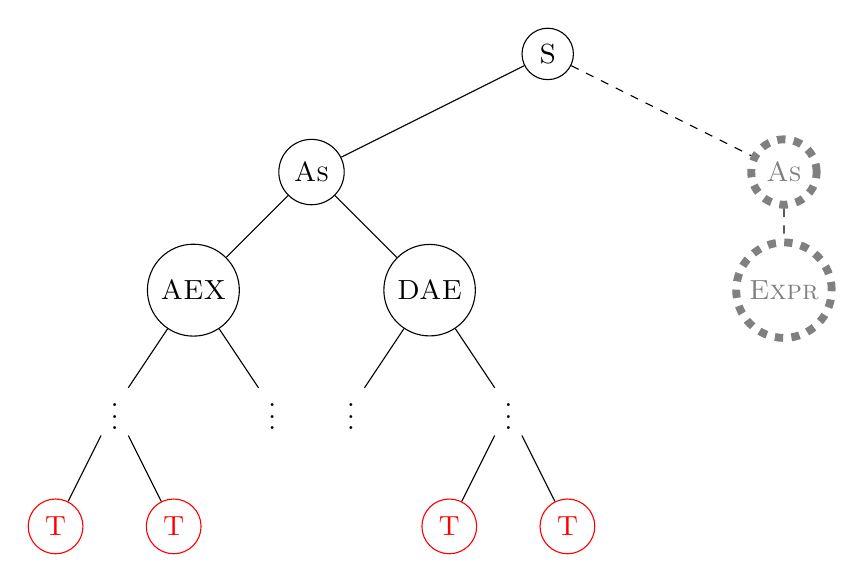
\begin{tikzpicture}[level/.style={sibling distance=60mm/#1}]
\node [circle,draw] (z){\textsc{S}}
  child {node [circle,draw] (a) {\textsc{As}}
    child {node [circle,draw] (b) {\textsc{AEX}}
      child {node {$\vdots$}
        child {node [circle,draw,color=red] (d) {\textsc{T}}}
        child {node [circle,draw,color=red] (e) {\textsc{T}}}
      } 
      child {node {$\vdots$}
      }
    }
    child {node [circle,draw] (g) {\textsc{DAE}}
      child {node {$\vdots$}}
      child {node {$\vdots$}
      child {node [circle,draw,color=red] (d) {\textsc{T}}}
        child {node [circle,draw,color=red] (e) {\textsc{T}}}
        }
    }
  }
%  child {node [circle,draw] (j) {\textsc{As}}
    child[dashed] {node [circle,draw,color=gray,line width=1mm] (k) {\textsc{As}}
        child {node [circle,draw,color=gray,line width=1mm] (l) {\textsc{Expr}}}
%    }
};
\end{tikzpicture}
 \caption{Sample \gls{CFG} transformation.}
    \label{fig:extended_cfg}
\end{figure}

\Cref{fig:extended_cfg} depicts an example of a transformation performed
on a section of the Kotlin grammar.
In this scenario, the root node \textsc{s} represents a \textit{statement} in the Kotlin
language and directly maps to a symbol in the core \gls{CFG}.
The symbol \textsc{s} could follow a production to sample an \textit{assignment}
node \textsc{as} as depicted in the left half of the figure.
This rule introduces additional semantic constraints, which the grammar omits.
The \textsc{as} node may be extended into either
an assignable expression (\textsc{aex}) or 
a directly assignable expression (\textsc{dae}), the details of which are
not important for the sake of this example.
Either production can in turn unravel into a chain of derivations that eventually
sample terminal nodes \textsc{t}.
Following this series of derivations, the semantic constraints that the production
$\textsc{s} \to \textsc{as}$ entails (such as type consistency in the assignment)
do not propagate to further links in the chain,
and thus the likelihood of generating
valid code by trivially sampling terminal nodes in the derivation
is vanishingly small.

The transformed grammar shown on the right branch of the \textsc{s} symbol circumvents
this problem by truncating the grammar at the node that introduces such constraints.
In this case, the algorithm transforms \textsc{as} node into its extended version,
which encodes relevant constraints within its \texttt{sample} property.
Transformed nodes may additionally transfer such constraints between them when sampled:
for instance, the assignment node may propagate its type-consistent constraint to a generic
\textsc{expr} node that generates constraint-aligned and valid Kotlin expressions.

This extended \gls{CFG} technique provides several advantages.
First, it forms a framework that solves the problem of semantically constrained grammar sampling.
By implementing the appropriate \texttt{sample} properties,
one can effectively evade the problems that the context-invariant grammar raises.
Second, it is an effective trade-off between implementation difficulty and core grammar usage. 
This technique preserves the key properties and relations in the Kotlin grammar, while
not necessitating that every production is individually catered to. 
For instance, transformed nodes may simply inherit part of
their structure or their entire specification from the \textsc{antlr4} definition.

Finally, the extended \gls{CFG} framework serves as a versatile foundation for fuzzing
algorithms, by allowing higher-level routines to target specific symbols in the grammar.
This property favors configurability and allows for extensive adaptations
of the core grammar.
Practitioners may additionally choose to sample only select nodes in the grammar,
thus effectively targeting desired subsets of the Kotlin language.
% This property may prove valuable as practitioners could use heuristics to stress 
% certain language features, compiler modules, or code bases in a more reliable
% manner than depending on sheer randomness.

This approach stands out from the current body of literature through 
the balance it strikes between the level of user "intervention" in re-writing grammar
rules and the utilization of pre-written grammar specifications.
In isolation, neither side of this trade-off is novel.
\textsc{Csmith} \cite{yang2011finding} has demonstrated the effectiveness
of manually constructing a sampling structure without
direct usage of a grammar over a decade ago, while approaches like
\textsc{ISLa} \cite{steinhofel2022input} show that
constraint-annotated grammars can effectively encode
common and meaningful semantic constraints.
However, our integration of contextual sampling within an extended
grammar representation enables algorithms built on top of it
to individually tune the semantic constraints of each
symbol, while always retaining to option to "fall back" on the 
pure grammar representation where appropriate, preserving the \textit{shape} of the grammar.
\subsection{\label{subsec:context-efcg} Connecting Context and Grammar}


To fully leverage their \texttt{sample} property, nodes in the 
extended grammar representation require an extensive connection to their local context.
To facilitate this arrangement, the we connect the initial (or \textit{root})
context to the node from which sampling starts.
As sampling algorithms recursively visit nodes in the extended grammar,
additional information embedded in each node helps the traversal decide
whether the current context should be transmitted as-is, cloned, or mutated.

Simple nodes like expressions utilize an unchanged context, while more complex
constructs, like variable declarations may insert additional identifiers.
Encompassing constructs like class and function definitions are scope sensitive,
which requires careful handling of local and nested operations.
To address this, each such node creates a local copy of the context, to
which it might add isolated information, before persisting globally accessible data
(i.e., function names, or new types) to the root context.
In essence, this integration allows for autonomous context-sensitive random sampling from the 
extended grammar: the extended nodes each query the context
in such a way that consistent constructs emerge.
The context, in turn, provides an interface that provides several guarantees with respect 
to future parameterized queries.

\section{\label{sec:repr} Code Representation}

To facilitate the implementation of measurable 
optimization criteria, we propose a versatile \gls{GA}-based framework
that supports common evolutionary search operators.
Such a framework requires a central representation of Kotlin code that is
granular enough to leverage the rich semantic information accessible through
the context, and simple enough to support large numbers of operator
calls during search.
To achieve this, we designed a hierarchical chromosomal representation
that distinguishes between three levels of separation.

The hierarchy roots itself in a tri-level
complexity abstraction that discerns between pieces of code
based on scope and isolated validity.
\Cref{fig:code-hierarchy} illustrates this hierarchy.
\textit{Fragments} lie at the base of the pyramid and compose low-level 
language constructs, such as expressions and statements.
These pieces of code do not capture any logic
structure and rely heavily on surrounding semantic context.
A step above are the code \textit{snippets}: individually encapsulated
pieces of code comprised of fragments.
Snippets emerge when changes in scope are significant enough to
merit a logical separation.
Such scenarios generally occur along the lines of \gls{OO} design,
and include functions, methods, and classes.


\begin{figure}[htp]
\centering
\begin{tikzpicture}[scale=0.55]
        \filldraw[very thick,white,fill=gray] (0,0) -- (-7.5,-9) -- (7.5,-9);
        \filldraw[very thick,white,fill=gray!60] (0,0) -- (-5,-6) -- (5,-6);
        \filldraw[very thick,white,fill=gray!30] (0,0) -- (-2.5,-3) -- (2.5,-3);
        \node at (0,-2) {\bfseries\sffamily\scshape\Large Block};
        \node at (0,-4.5) {\bfseries\sffamily\scshape\Large Snippet};
        \node at (0,-7.5) {\bfseries\sffamily\scshape\Large Fragment};
        \node[text width=8cm] at (10,-2) {\Large $\bullet$ compilable, independent};
        \node[text width=8cm] at (12.5,-4.5) {\Large $\bullet$ interdependedent};
        \node[text width=8cm] at (14.5,-7.5) {\Large $\bullet$ unstructured};
    \begin{scope}[xshift=-3.7cm,yshift=-3cm]
        \draw[-{Triangle[width=18pt,length=12pt]}, line width=8pt, rounded corners=10pt, black] (-0.75,0) -- (-0.75,1) -- (2,1);
        \node[text width=5cm] at (2.75,-.5) {\small matching};
    \end{scope}
    \begin{scope}[xshift=-5.7cm,yshift=-5.5cm]
        \draw[-{Triangle[width=18pt,length=12pt]}, line width=8pt, rounded corners=10pt, black] (-1,0) -- (-1,1) -- (2,1);
        \node[text width=5cm] at (2,-.5) {\small aggregation};
    \end{scope}
\end{tikzpicture}

 \caption{Representational hierarchy of code complexity abstractions.}
 \label{fig:code-hierarchy}
\end{figure}

Snippets serve as an intermediate layer that captures sufficient information to be individually actionable (i.e., a function that can be called), but not enough to be
context-independent.
The interdependency of snippets materializes as a consequence of
the sequential nature of node sampling: as nodes recursively unfold
their \texttt{sample} property, prior changes to the context
trigger subsequent consequences (i.e., previously generated 
functions may appear in later expressions).
To overcome this obstacle several snippets can assemble into \textit{blocks},
the highest construct of the pyramid.
This snippet \textit{aggregation} procedure works on the basis of a dependency matching
algorithm that recursively traverses snippets within a Kotlin file and retrieves
external snippets that their fragments depend on.

The pyramidal abstraction construct shares conceptual similarities with both
the works of \citet{holler2012fuzzing} and \citet{han2019codealchemist}.
However, there are fundamental differences between our method and past work.
Unlike \citet{holler2012fuzzing}, more sophisticated, language-targeted
generation procedures serve as the basis of novel code blocks, which do not
rely on input seed programs.
The aggregation of snippets into blocks also differs from the semantics-aware
assembly proposed by \citet{han2019codealchemist}, which infers language constraints
from a corpus of over 200,000 files.
Our approach requires no such input, making the generation process entirely self-sustaining. 

\Cref{fig:blocks} exemplifies the differences between the three levels
of the hierarchy.
The statements in lines 2 and 6, as well as the expression
in line 10 are all instances of \textit{fragments}: pieces
of code that too small to track in the model.
The functions \texttt{x}, \texttt{y}, and \texttt{z} are all \textit{snippets}:
independently separable pieces of code that are not necessarily self-sufficient.
Finally, there are three \textit{blocks} in this example: $\langle \texttt{x} \rangle$,
$\langle \texttt{x}, \texttt{y} \rangle$,
and $\langle \texttt{x}, \texttt{y}, \texttt{z} \rangle$.
All three of these blocks share the property that they are context-independent:
the dependencies for all snippets in the block are also part of the block.
Preserving this property during search is critical not only because it is the most
effective way of employing the context's semantic guarantees,
but also because it ensures that compiler resources do not go to waste
in analyzing incomplete files.
The \textit{block} abstraction is the cornerstone of the 
\gls{GA} framework, shaping all higher-level operators and constructs.
In the remainder of this section, we analyze the foundational elements of
the evolutionary fuzzing toolkit.

\begin{figure}
\begin{lstlisting}[language=Kotlin]
fun x() : Double {
	return 0.0
}

fun y() : Double {
	return x() + 1.0
}

fun z() {
	return y()
}
\end{lstlisting}
\caption{Illustration of fragments, snippets, and blocks.}
\label{fig:blocks}
\end{figure}

\paragraph{Individuals.} The population of the \gls{GA} consists
of individual \textit{blocks} encoded in a chromosomal representation as follows.
A chromosome consists of a list $\mathcal{L}$ of triples
$\mathcal{S} := \langle \mathcal{R}, \mathcal{D}, \mathcal{T} \rangle$ representing snippets,
with $\mathcal{R}$ a representation of the signature of the snippet,
$\mathcal{D}$ a list of signatures of snippets that $\mathcal{S}$ depends on,
and $\mathcal{T}$ the text that the snippet contains.
Considering again the code in \Cref{fig:blocks},
the chromosome encoding the block $\langle \texttt{x}, \texttt{y} \rangle$
is $\mathcal{L}_{\langle \texttt{x}, \texttt{y} \rangle} =
[ \langle
\texttt{x} : \lambda \to \texttt{Double}, \emptyset, \mathcal{T}_{\texttt{x}}\rangle,
\langle \texttt{y} : \lambda \to \texttt{Double},
\{ \texttt{x} : \lambda \to \texttt{Double} \}, \mathcal{T}_{\texttt{y}} \rangle ]$
The first entry in the list models the \texttt{x} function, with a
$\lambda$-calculus inspired signature, an empty dependency set, and
the first lines 3 of the code.
The second entry is analogous, except for the dependency set 
that contains the signature of \texttt{x}, signaling that
lines of code 5-7 require the presence of \texttt{x} for completeness.

\paragraph{Context-Aware Partitioning.} A downside of the
established chromosome model has to do with the ordering of
snippets inside $\mathcal{L}$.
Though representationally irrelevant, the order of snippets within
the list becomes crucial when the chromosome instantiates
a concrete piece of code.
Snippets in Kotlin can be order-sensitive, meaning that to
instantiate valid code, the list of snippets within the chromosome
should be arranged such that a topological dependency structure
emerges.
Using again the example in \Cref{fig:blocks}, this means
that within the chromosome representing the entire piece of code,
the snippet \texttt{x} must always be precede \texttt{y} and \texttt{z}.
Similarly, \texttt{y} must always appear before \texttt{z}.

There are several ways to achieve this ordering.
Since the generative process is iterative, the first instantiation
of a block always obeys this constraint.
However, preserving this property during the application of
variation operators proves more challenging.
To effectively mutate and recombine individuals,
blocks require the capability of
identifying entire dependency structures centered around particular snippets.
In other words, given a snippet \texttt{s} present in a block
\texttt{b}, \texttt{b} should be able to  identify a \textit{partition}
of itself that includes (i) \texttt{s}, (ii) all snippets
that depend on \texttt{s}, and (iii) all downstream dependencies of (i) and (ii).
We refer to a partition that such a structure as a \textit{self-sufficient} partition
of a block.

To build such a partition starting from an arbitrary snippet
requires careful analysis of the dependency structure within a block.
To implement this, we propose a technique that models the
structure of a block as a \textit{dependency graph}, a common
data structure used in static analysis of programs.
Each node \texttt{n} represents a snippet within the block,
and each directed edge $\texttt{n}_1 \to \texttt{n}_2$
denotes that snippet $\texttt{n}_1$ depends on $\texttt{n}_1$.
To construct a self-sufficient partition starting from a node $\texttt{n}$,
we employ two procedures that traverses the dependency graph
to gather information regarding its topology.
An \textit{upstream} traversal starting at \texttt{n} walks
along every possible path \textit{ending} in \texttt{n}, in
effect gathering all blocks that either directly or indirectly depend on \texttt{n}.
Reflexively, a \textit{downstream} traversal beginning at \texttt{n}
walks on every path originating in \texttt{n} and gathers all of \texttt{n}'s
dependencies.

\Cref{fig:traversals} depicts several sample traversals of a
snippet dependency structure similar to that introduced in \Cref{fig:blocks}.
Nodes with thick borders are affected by the traversal, while thinly bordered ones are not.
Black depicts that the node is the starting point of the traversal,
while blue and red denote nodes selected during up- and downstream traversals, respectively.
Subfigure (a) gives the standalone topology of the block, and selects
snippet \texttt{y} as the root of the traversal.
An upstream traversal rooted in \texttt{y} would select \texttt{b} and \texttt{z},
which directly depend on \texttt{y}, as depicted in panel (b).
A downstream traversal rooted in \texttt{y} would additionally yield
snippet \texttt{x}, which is \texttt{y}'s only direct dependency, as shown in 
subfigure (c).
Finally, it is important to note that the repeated application of up- and downstream
traversal on increasingly larger sets of nodes (i.e., each traversal considers \textit{all}
nodes returned by the previous) yields the largest connected subgraph containing the
original starting node.
Subfigure (d) illustrates three such traversals:
starting at \texttt{a}, \texttt{b} is selected during an upstream traversal.
Next, \texttt{y} and \texttt{x} from the downstream traversal rooted at \texttt{b}.
Lastly, an upstream traversal rooted at either \texttt{x} or \texttt{y} yields \texttt{z}.
The additional benefit of traversals is that they preserve
the ordering of nodes in graph, which graph walking algorithms may fail to do.

\begin{figure}[t!]
\centering
\subfigure[Initial choice of snippet.]{
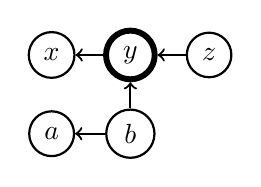
\begin{tikzpicture}[node distance={10mm}, thick, main/.style = {draw, circle}] 
\node[main] (1) {$x$}; 
\node[main, line width=0.75mm] (2) [right of=1] {$y$}; 
\node[main] (3) [right of=2] {$z$}; 
\node[main] (4) [below of=1] {$a$}; 
\node[main] (5) [right of=4] {$b$};  
\draw[->] (2) -- (1);
\draw[->] (3) -- (2);
\draw[->] (5) -- (2);
\draw[->] (5) -- (4);
\end{tikzpicture}}
\hfill
\subfigure[Upstream traversal from node \texttt{y}.]{
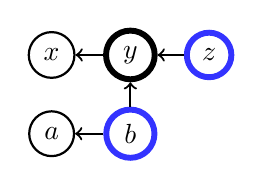
\begin{tikzpicture}[node distance={10mm}, thick, main/.style = {draw, circle}] 
\node[main] (1) {$x$}; 
\node[main,line width=0.75mm] (2) [right of=1] {$y$}; 
\node[main,draw=blue!80,line width=0.75mm] (3) [right of=2] {$z$}; 
\node[main] (4) [below of=1] {$a$}; 
\node[main,draw=blue!80,line width=0.75mm] (5) [right of=4] {$b$};  
\draw[->] (2) -- (1);
\draw[->] (3) -- (2);
\draw[->] (5) -- (2);
\draw[->] (5) -- (4);
\end{tikzpicture}
}
\hfill
\subfigure[Successive downstream traversal from node \texttt{y}.]{
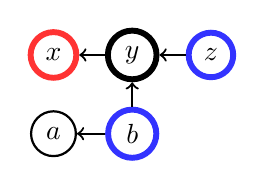
\begin{tikzpicture}[node distance={10mm}, thick, main/.style = {draw, circle}] 
\node[main,draw=red!80,line width=0.75mm] (1) {$x$}; 
\node[main,line width=0.75mm] (2) [right of=1] {$y$}; 
\node[main,draw=blue!80,line width=0.75mm] (3) [right of=2] {$z$}; 
\node[main] (4) [below of=1] {$a$}; 
\node[main,draw=blue!80,line width=0.75mm] (5) [right of=4] {$b$};  
\draw[->] (2) -- (1);
\draw[->] (3) -- (2);
\draw[->] (5) -- (2);
\draw[->] (5) -- (4);
\end{tikzpicture}
}
\hfill
\subfigure[Successive up-, down-, and upstream traversals starting at \texttt{a}.]{
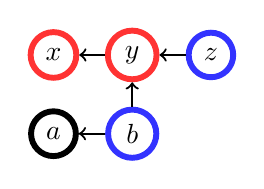
\begin{tikzpicture}[node distance={10mm}, thick, main/.style = {draw, circle}] 
\node[main,line width=0.75mm,draw=red!80] (1) {$x$}; 
\node[main,line width=0.75mm,draw=red!80] (2) [right of=1] {$y$}; 
\node[main,line width=0.75mm,draw=blue!80] (3) [right of=2] {$z$}; 
\node[main,line width=0.75mm] (4) [below of=1] {$a$}; 
\node[main,line width=0.75mm,draw=blue!80] (5) [right of=4] {$b$};  
\draw[->] (2) -- (1);
\draw[->] (3) -- (2);
\draw[->] (5) -- (2);
\draw[->] (5) -- (4);
\end{tikzpicture}
}
\caption{Sample upstream and downstream traversals of snippet dependencies. }
\label{fig:traversals}
\end{figure}

\paragraph{Mutation.} To fully take advantage of the properties of blocks,
mutation operators must ensure the preservation self-sufficiency.
Since perturbing the dependency hierarchy within blocks
would render any validity guarantees pointless, we designed
mutation procedures to operate on partitions of code blocks selected by 
means of the previously established traversals.
This includes three mutation varieties:

\begin{itemize}
	\item \textbf{Removal} of a selected partition. This operator first chooses a random 
	snippet within the block and performs an upstream traversal from that snippet.
	The operator then removes all collected snippets from the chromosome.
	\item \textbf{Context-Free Addition} performs a sample operation
	on the node that the given block originates from, and appends the result to the end
	of the chromosome.
	\item \textbf{Context-Aware Addition} first brings the context in a state
	that is compatible with the block subject to mutation, and then performs a sample
	operation. The result extends the chromosome as in the context-free case.
\end{itemize}

\paragraph{Recombination.} We propose a simple recombination operator
that takes in a pair of chromosomes $\mathcal{L}_{p_1}$ and $\mathcal{L}_{p_2}$
and creates two offspring  $\mathcal{L}_{o_1}$ and $\mathcal{L}_{o_2}$.
The offspring start out as identical copies of each parent, before
crossover swaps two collections of snippets between them.
The collection of snippets emerges using repeated up- and downstream
traversals initially rooted a randomly chosen snippet in the block.
The resulting selections preserve both the self-sufficiency and
ordering constraints of both the extracted and remaining partitions.
As a result, the selected partitions of each block are swapped and appended
to the opposite chromosome.

\paragraph{Selection.} We provide standard selection operators for both
single- (tournament and proportionate selection) and
multi-/many-objective (domination rank and domination count selection) fitness functions.
\\\\
To exploit the power of this framework to its full extent,
we allow for a large degree of external configuration.
The remainder of this section covers three meta-heuristic
strategies implemented on top of this general framework and analyzes
their merits and potential.


\section{\label{sec:heuristics}Generative Heuristics}

The semantic, syntactic, and representational interfaces
described in Sections \ref{sec:context}, \ref{sec:syntax}, and \ref{sec:repr}
lay the foundation for more complex overarching heuristics
to guide a generative process underlying fuzzing.
This section explores three meta-heuristic guiding oracles shaped into
several concrete algorithm variations and their application
in the context of compiler fuzzing.
Subsection \ref{subsec:random-sampling} establishes a standard baseline algorithm,
while \Cref{subsec:diversity-ga}, and \ref{subsec:proximity-ga}
elaborate on two more complex heuristic approaches,
centering on syntax and semantics, respectively.

\subsection{\label{subsec:random-sampling} Random Sampling}

\newacronym{RS}{RS} {Random Sampling}

Perhaps the simplest method to leverage the context and grammar constructs
is to repeatedly sample a given node in the extended grammar by traversing
context-informed random paths.
We refer to this generative procedure as \Gls{RS}.
Though trivial in its scope, this approach has proven deceptively powerful
and is the dominant search strategy employed in some shape by all state-of-the-art
fuzzers discussed in \Cref{sec:compiler_testing}.
Despite its simplicity, \gls{RS} establishes a powerful interface, which
all algorithms involved in this study follow.
\Cref{alg:rs} describes the \gls{RS} procedure.

\begin{algorithm}

	\SetKwData{Left}{left}
	\SetKwData{This}{this}
	\SetKwData{Up}{up}
	\SetKwFunction{init}{InitializeAndEvaluatePopulation}
	\SetKwFunction{terminate}{ShouldTermiante}
	\SetKwFunction{offspring}{CreateAndEvaluateOffspring}
	\SetKwFunction{select}{SelectIndividuals}
	\SetKwFunction{time}{TimeElapsed}
	\SetKwFunction{clone}{Clone}
	\SetKwFunction{sample}{Sample}
	\SetKwInOut{Input}{Input}
	\SetKwInOut{Output}{Output}
	\Input{Node to sample $\mathcal{N}$, Context $\mathcal{C}$, Time Budget $s$}
	\Output{Collection of generated Kotlin files}
	\BlankLine
	\DontPrintSemicolon
	%\emph{special treatment of the first line}\;
	$A \gets \emptyset$\;
	\While{$\neg$ \time{$s$}}{
		$c \gets \clone {$\mathcal{C}$}$\;
		$b \gets \sample {$\mathcal{N}$, c}$\;
		$A \gets A \cup \{ b \}$\;
	}
	\Return $A$\;

	\caption{Random Sampling}
	\label{alg:rs}
\end{algorithm}


The sampling procedure takes as input a node $\mathcal{N}$ of the extended Kotlin \gls{CFG}
, a context $\mathcal{C}$, 
and a time budget $s$ that determines how long to run for.
The loop simply invokes the $\mathcal{N}$'s \texttt{sample} property repeatedly,
generating code that is syntactically rooted in the target.
Since this procedure mutates the provided context, the main loop creates a fresh
clone of original context $\mathcal{C}$ to prevent cross-referencing between
different files.
An archive $A$ tracks and collects each generated file,
and is returned once the allotted time has exhausted.

% The proven effectiveness of random sampling as a generative mechanism
% in conjunction with a \gls{BB} treatment of the target compiler
% has lead researchers to focus on developing auxiliary methods
% in support of the core random search driving mechanism.
As a result of the prevelance of \gls{RS} in conjunction with a \gls{BB} treatment of
the compiler under test, many of today's compiler fuzzing tools utilize heuristics to shape
the direction of stochastic sampling procedures rather than directly
optimize solutions under concrete objectives.
The remainder of this chapter explores auxiliary optimization settings,
that seek to substitute the standard \gls{RS} procedure
with directly measurable objective functions, as an alternative
paradigm to unguided sampling.

\subsection{\label{subsec:diversity-ga}Syntactic Diversity-Driven Search}

Generating code that covers a broad range of the Kotlin
input space is a key challenge for thoroughly exercising the many features
of the compiler.
This subsection delves into two ways a \gls{GA} can model, measure,
and optimize for the diversity of its generated files, with the goal
of triggering varied internal compiler behavior.

\subsubsection{\label{subsec:model-div} Modeling Syntactic Diversity} Diversity is intrinsically linked to the
concept of (dis)similarity.
To effectively build such a notion in the domain of semantically
complex Kotlin code, the fuzzer requires a transformation capable
of mapping Kotlin blocks to a space embedded with
a notion of distance.
For this purpose, we opted to measure the number of distinct
language constructs that each block contains.
To this end, the grammar sampling process actively tracks
its stochastic traversal of the \gls{CFG} graph such that
each new occurrence of a node causes a dedicated counter to increment.

Once generation has concluded, the newly established block
internally maintains a vectorized numerical representation of
all its counters.
This simplified representation implicitly describes a 
coordinate space that contains every possible valid piece of Kotlin code
(though, clearly, this mapping is surjective as many pieces of code
may be mapped to identical points).
Furthermore, this syntactically-minded space largely overlooks
the semantic nuances of the blocks that inhabit it, driving the genetic process
almost entirely through the \gls{CFG}.
This is key for promoting structurally diverse blocks in the population.

\newacronym{SO}{SO} {Single-Objective}

\subsubsection{\label{subsec:soga}Direct Single-Objective Diversity Optimization}

We integrate the
diversity model into the \gls{GA} framework by means of a custom \gls{SO} fitness function.
Let $b_1$ and $b_2$ be two code blocks, generated using the procedure
described in the previous paragraphs.
Let $m : \mathcal{B} \to \mathbb{N}^{k}$ be the mapping that operates
on the input space of all possible blocks $\mathcal{B}$ and outputs
a $k$-dimensional vector of natural numbers representing, for each position,
the number of language structures of a certain type present within the block.
Using this mapping, any common measure of distance
$d : \mathbb{N}^k \times \mathbb{N}^k \to \mathbb{R}$ (i.e., Euclidean) may be used to determine
the distance between two blocks.
Within this setting, we equate the notion of similarity
the distance between two blocks.
From these conventions, the notion of population-wide 
dissimilarity follows:

\begin{equation}
dis(b, P) = min_{b^{(i)} \in P - \{ b \}} \{ d(m(b), m(b^{(i)})) \}
\label{eq:sim}
\end{equation}


Intuitively, the dissimilarity of a block $b$ with regard to a population
$P$ is the minimum distance from $b$ to a different block $b^{(i)}$
belonging to the population. 
This notion gives rise to a population-wide diversity fitness function:

\begin{equation}
\min_{b \in \mathcal{B}} f^{(SO)}_{\texttt{DIV}}(b, P) = \frac{1}{1 + dis(b, P)}
\end{equation}

\begin{algorithm}[t]

	\SetKwData{Left}{left}
	\SetKwData{This}{this}
	\SetKwData{Up}{up}
	\SetKwFunction{init}{InitializeAndEvaluatePopulation}
	\SetKwFunction{terminate}{ShouldTermiante}
	\SetKwFunction{offspring}{CreateAndEvaluateOffspring}
	\SetKwFunction{select}{SelectIndividuals}
	\SetKwFunction{time}{TimeElapsed}
	\SetKwFunction{clone}{Clone}
	\SetKwFunction{sample}{Sample}
	\SetKwInOut{Input}{Input}
	\SetKwInOut{Output}{Output}
	\Input{Population size $n$, Node to sample $\mathcal{N}$, Context $\mathcal{C}$, Time Budget $s$}
	\Output{Collection of generated Kotlin files}
	\BlankLine
	\DontPrintSemicolon
	$t \leftarrow 1$\;
	$P_1 \leftarrow $ \init{$n, \mathcal{N}, \mathcal{C}$}\;
	$P^{*} \leftarrow P_1$\;
	\While{$\neg$ \time{$s$}}{
		$O_t \leftarrow$ \offspring {$P_t$}\;
		$P_{t+1} \leftarrow$ \select{$P_{t}, O_{t}, f^{(SO)}_{\texttt{DIV}}$}\;
		\If{$\sum_{b\in P_{t+1}} f^{(SO)}_{\texttt{DIV}}(b, P_{t+1}) > \sum_{b\in P^{*}} f^{(SO)}_{\texttt{DIV}}(b, P^{*})$} {
		$P^{*} \leftarrow P_{t+1}$\;
		}
		$t \leftarrow t + 1$\;
	}
	\Return $P^{*}$

	\caption{Single-Objective Diversity Genetic Algorithm}
	\label{alg:sodga}
\end{algorithm}


This formulation inverts and normalizes the similarity metric, meaning that
$f^{(SO)}_{\texttt{DIV}}$ has reached an optimum when $dis(b, P)$ has reached its maximum.
In other words, the higher the minimum distance from a block to its population peers is,
the better its fitness.
While the notions of (dis)similarity and diversity allow for different computations,
the one put forward in \Cref{eq:sim} fits the purposes of compiler fuzzing
especially well.
Because the fitness of the individual is determined on the basis of its \textit{most similar}
counterpart, this evaluation method decreases the likelihood of preserving blocks
that are very similar to other individuals.
\Cref{alg:sodga} sketches the \gls{GA} incorporating this fitness criterion.

Other methods of determining similarity (such as, for example, the \textit{mean}
distance to the rest of the population) do not maintain this property as well,
since blocks that map farther away in the mapping space might significantly
improve the fitness of several blocks that are very similar to each other, but
dissimilar from the rest of the population.

 \newacronym{MO}{MO} {Many-Objective}

\subsubsection{\label{subsec:moga}Indirect Many-Objective Diversity Optimization}

Though it models the concept of inter-block syntactic similarity well,
the \Gls{SO} optimization criterion suffers from one key limitation.
$f^{(SO)}_{\texttt{DIV}}$ fails to faithfully depict
the entire similarity landscape, implicitly requiring
a trade-off in importance between similarity
to close (or similar) and far away (or dissimilar) blocks.
The higher the weight on the local topology, the more likely it is for the \gls{SO} formulation to "miss" the global landscape.
The converse is also true, requiring the algorithm design to carefully strike
a balance between the two conflicting objectives.
Within the scope of compiler fuzzing, such a balance is very challenging to reason about,
not least because the key to unlocking a balanced fitness criterion
rests on many layers of abstractions and tools,
all centered around the compiler.

To overcome this limitation, we propose a second method
of obtaining a diverse set blocks, centered around a \Gls{MO}
interpretation of diversity. 
Let $f_l(b) : \mathcal{B} \to \mathbb{N}, \forall l \in \mathbb{L}$ be
a function that maps arbitrary blocks to a natural number
equal to the number of occurrences of language construct $l$
in the input block, with $\mathbb{L}$ the set of all valid language constructs
of Kotlin.
In addition, let $f_{sz}(b) : \mathcal{B} \to \mathbb{N}$ be a function
that maps input blocks to their size.
There are multiple sensible choices for the measurement of block size, but in this
study we limit our measurements to a single metric that counts the number of characters
in the text representation of the individual.
Altogether, these functions give rise to a novel \gls{MO} objective function:

\begin{equation}
\max_{b \in \mathcal{B}} f^{(MO)}_{\texttt{DIV}}(b) = \left\lbrace -f_{sz}(b), ~f_{l_1}(b),~f_{l_2}(b),~\dots,~f_{l_n}(b)|~l_i \in \mathbb{L} \right\rbrace
\end{equation}

Within this formulation, $f^{(MO)}_{\texttt{DIV}}$ attempts to simultaneously
\textit{maximize} the number of each language feature
and \textit{minimize} the size of each block.
In essence, this gives rise to a Pareto frontier of blocks
that have a high number of different combinations sets of language features
within a limited size.
The size minimization is an essential ingredient to this interpretation of diversity.
Omitting the size objective causes $f^{(MO)}_{\texttt{DIV}}$
to simply maximize the number of each language feature independently.
In practice, this is a poor decision for two key reasons.

First, the nature of language feature objectives is strictly linear and additive.
Since larger blocks contain more code, they also contain, by extension, more
language features on average.
This causes larger blocks to be (on average) much more likely
to Pareto dominate smaller blocks and take over the population very quickly.
This setting would heavily favor larger blocks, entirely missing
the enveloping goal of optimization.
Second, exploring a search space composed of smaller blocks may uncover
more valuable compiler defects.
Smaller blocks not only make it easier to pinpoint the cause of the
uncovered faults, but are also more likely to lead to
more impactful faults: the smaller the code pertaining to a compiler bug,
the more generalizable and likely it is to appear in real-world projects.

\begin{algorithm}[t]

	\SetKwData{Left}{left}
	\SetKwData{This}{this}
	\SetKwData{Up}{up}
	\SetKwFunction{init}{InitializeAndEvaluatePopulation}
	\SetKwFunction{terminate}{ShouldTermiante}
	\SetKwFunction{offspring}{CreateAndEvaluateOffspring}
	\SetKwFunction{select}{DominationSelection}
	\SetKwFunction{time}{TimeElapsed}
	\SetKwFunction{processarchive}{ProcessNewArchiveEntries}
	\SetKwFunction{initarchive}{InitializeElitistArchive}
	\SetKwFunction{sample}{Sample}
	\SetKwInOut{Input}{Input}
	\SetKwFunction{shuffle}{Shuffle}
	\SetKwInOut{Output}{Output}
	\Input{Population size $n$, Node to sample $\mathcal{N}$, Context $\mathcal{C}$, Time Budget $s$}
	\Output{Collection of generated Kotlin files}
	\BlankLine
	\DontPrintSemicolon
	$A \leftarrow$ \initarchive{$f^{(MO)}_{\texttt{DIV}}$}\;
	$t \leftarrow 1$\;
	$P_1 \leftarrow $ \init{$n, \mathcal{N}, \mathcal{C}$}\;
	\While {$\neg$ \time{$s_t$}}{
		$A \leftarrow$ \processarchive{$P_t, f^{(MO)}_{\texttt{DIV}}$}\;
		$O_t \leftarrow$ \offspring {$P_t$}\;
		$P_{t+1} \leftarrow$ \select{$P_{t}, O_{t}, f^{(MO)}_{\texttt{DIV}}$}\;
		$t \leftarrow t + 1$\;
	}
	\Return $A$\;
	\caption{Many-Objective Diversity Genetic Algorithm}
	\label{alg:modga}
\end{algorithm}

\Cref{alg:modga} contains the pseudocode for the \gls{MO} optimization
algorithm based on $f^{(MO)}_{\texttt{DIV}}$.
It is a straight-forward extensions of \gls{SO} \gls{GA} that utilizes
an archive (lines 1, 5) to track the set of non-dominated solutions
that together comprise the approximation set.
With each iteration, the archive could both grow (by inserting new non-dominated
blocks) and shrink (by discarding older individuals dominated by newer additions).
The algorithm returns this approximation set as its final output (line 9).

\begin{figure}[t!]
\centering
\subfigure[Initial distribution of code blocks in the syntactic similarity space.]{
\includegraphics[scale=0.27]{img/diversity_all.png}
}
\hfill
\subfigure[Truncated selection of individuals based on $f^{(SO)}_{\texttt{DIV}}$.]{
\includegraphics[scale=0.27]{img/diversity_so_selection.png}
}
\hfill
\subfigure[Selection of individuals using domination rank and $f^{(MO)}_{\texttt{DIV}}$ without the size component.]{
\includegraphics[scale=0.27]{img/diversity_mo_selection.png}
}

\caption{Illustration of different optimization criteria behavior in the diversity space.}
\label{fig:diversity}
\end{figure}

\subsubsection{\label{subsec:diversity-example}Differences in Diversity Nuance}

Grasping implications of the different diversity formulations
may prove tricky.
To help build intuition regarding how the selection
criteria and their respective formulations
impact the landscape of the search process, we provide an example in \Cref{fig:diversity}.
Subfigure (a) shows a population of 30 points, the features of which
were each drawn from categorical uniform distributions.
In practice, the axes represent the number of language
features (statements, functions, etc.)
each individual (block) exhibits.
Within this space, the choice of modeling heuristic drastically affects
which blocks get selected to the next round of the algorithm.

Consider a scenario in which $f^{(SO)}_{\texttt{DIV}}$ is the fitness criterion,
and the algorithm uses a simple truncation selection method
to determine the survivors to the next generation.
In this case, the selection operator favors
blocks that are the farthest away
from any other blocks in the population, as subfigure (b) depicts.
The points depicted by black crosses are the ones
who survive the selection round.
While this mechanism does well to identify 
portions of the search space which the population
sparsely inhabits, it is prone to "forgetting"
areas of high density that do not contribute to the selection.
This issue resembles the problem of \textit{front degradation}
in traditional \Gls{MO} evolutionary computation.
The populaiton-wide retention mechanism of the \gls{SO} diversity
\gls{GA} seeks to combat this.

Alternatively, consider the \gls{MO} setting, in which
the algorithm carries out selection by means
of truncation based on the domination rank of the individual.
This combination of operators results in the selection depicted
in subfigure (c).
Points depicted in black are selected, and the shape of the point
depicts its domination rank.
Within this pure maximization framework, the problem makes itself apparent:
points depicting blocks that are larger drastically diminish the probability
of smaller blocks (mapped to the bottom-left quartile of the figure) propagating
to the next round of the algorithm.
It is for this reason that $f^{(MO)}_{\texttt{DIV}}$ contains a size component
that aims to circumvent this obstacle and allow for a more even
distribution of individuals.

Notably, only one selection overlaps between
the two selection mechanisms proposed here.
Within the scope of compiler testing, it is extremely difficult
to analytically reason about which
formulation is better suited for uncovering defects.
For this reason, we set out to empirically analyze both
formulations within this study.

\subsection{\label{subsec:proximity-ga}Semantic Proximity-Driven Search}

Syntactic analysis alone cannot paint a sufficiently
detailed picture for comparing blocks.
While effective as a means of measuring the structural composition of
blocks, the syntactic diversity criteria introduced in the previous
section fail capture the semantic nuances of generated code.
In this subsection, we introduce a slew of techniques culminating in three
complementary \gls{GA} formulations that seek to better
account for the indispensable semantic dimension of Kotlin code. 

\subsubsection{Modeling Semantic Proximity}

Strictly speaking, the mathematical requirements to effectively
measure the semantic similarity between two blocks
are the same as those that syntactic diversity requires:
a sound mapping from the domain of code, and a measure of distance
in the mapped space.
However, the multifaceted nature of Kotlin semantics
present difficulties that syntactic models do not face.
The \textsc{antlr4} \gls{CFG} implementation that the Kotlin
developer team supplies as part of the language specification
condenses the rules of the language in a structured and processable
manner.
This reduces the complexity of interpreting the syntactic similarity
of two blocks down to assessing their relation with respect to the grammar.
Unfortunately, no such construct exists for the semantic counterpart of Kotlin.

\newacronym{ML4SE}{ML4SE} {Machine Learning for Software Engineering}
\newacronym{ML}{ML} {Machine Learning}
\newacronym{NLP}{NLP} {Natural Language Processing}
\newacronym{NN}{NN} {Neural Network}

To address this problem, we turn to techniques used in the field
of \Gls{ML4SE}.
Ever since \citet{hindle2016naturalness} shared their findings on the
high regularity of code in 2016, the field of \gls{ML4SE} has experienced a boom
in popularity and development.
Crucially, the study suggested that software regularity 
emerging from a property the authors call \textit{naturalness}, as opposed to syntax.
Since then, researchers adapted, tuned, and extended techniques
at the intersection of \gls{ML} and \gls{NLP} and successfully applied
them at scale for common software engineering tasks.
Non-trivial chores previously exclusively reserved for developers could now
be at least in part automated at scale through new \gls{ML4SE} techniques.

Of particular interest to our research is a class of models
that use an internal numeric representation of pieces of code
to simultaneously model both the syntax and the semantics of the input.
These models largely rely on architectures revolving around a \gls{NN}
trained on one or more tasks, generally involving both code and natural language.
In \gls{NLP} research, the (lower-dimensional) numeric representation of token-represented
input is referred to as an \textit{embedding}.

Embeddings exhibit two key properties that make them suitable candidates for the goals
of our optimization framework.
Though impossible to interpret in isolation, embeddings retain
an interpretation of the textual representation fed into them.
We specifically select embedding mechanisms that have been trained
in an end-to-end fashion using multimodal training criteria, in the hope
of taking advantage of the generalizability of such approaches.
Second, by populating a space with the embeddings of Kotlin code,
the notion of \textit{proximity} can simply be expressed by means
of a distance metric in the projected domain.

\begin{figure}[t]
\vspace{2cm}
\centering
\begin{tikzpicture}[transform canvas={scale=1.0},node/.style={circle, draw, thick}]

\foreach \Z in {0,0.5,1,1.5}
 {\draw[fill=gray,draw=black] (-8,0,\Z) rectangle (-7.25,1,\Z);}

\node[] at (-7.5,1.5)   (a) {Chromosome};

 \draw [-stealth] (-7.15, 0.5) -- node[pos=0.5,above]{Construct} (-5.5, 0.5);
 
 \pgfmathsetmacro{\cubex}{1.25}
\pgfmathsetmacro{\cubey}{1.25}
\pgfmathsetmacro{\cubez}{1.25}
\draw[black,fill=gray] (-4,1,0) -- ++(-\cubex,0,0) -- ++(0,-\cubey,0) -- ++(\cubex,0,0) -- cycle;
\draw[black,fill=gray] (-4,1,0) -- ++(0,0,-\cubez) -- ++(0,-\cubey,0) -- ++(0,0,\cubez) --  cycle;
\draw[black,fill=gray] (-4,1,0) -- ++(-\cubex,0,0) -- ++(0,0,-\cubez) -- ++(\cubex,0,0) -- cycle;

\node[] at (-4.25,1.875)   (a) {Text};

\draw [-stealth] (-3.25, 0.5) -- node[pos=0.5,above]{NN Input} (-1.75, 0.5);

  \foreach \y in {1,...,3}{
      \node[node] (i\y) at (-1,\nodesep*\y-0.5) {};
      \node[node, right=\layersep of i\y] (h1\y) {};
      \node[node, right=\layersep of h1\y] (h2\y) {};
    }

  \foreach \source in {1,...,3}
  \foreach \dest in {1,...,3}{
      \path[-stealth, thick] (i\source) edge (h1\dest);
      \path[-stealth, thick] (h1\source) edge (h2\dest);
    }

\draw[] (-1.5, -0.5) rectangle (1.25, 1.5);

\node[] at (-0.125,1.875)   (a) {Embedding NN};

\draw [-stealth] (1.5, 0.5) -- node[pos=0.5,above]{NN Output} (3.5, 0.5);

\node[right,scale=0.9] at (3.5,0.5)
    {$\begin{pmatrix}
        0.4\\[0.3em]
        0.2\\
        \vdots \\
        0.7
       \end{pmatrix} \in \mathbb{R}^{k}$};
      
%\draw [-stealth] (4.25, 0.25) -- (5.5, 0.25) -- (5.5,-0.45);


  \def\rvec{.8}
  \def\thetavec{30}
  \def\phivec{60}
  
  \draw[-stealth] (4.75, -0) -- (6.5, -0);
  
  % AXES
  \coordinate (O) at (8,-0,0);
  \draw[thick,->] (7,-0,0) -- (8,0,0) node[below left=-0.5]{$x$};
  \draw[thick,->] (7,-0,0) -- (7,1,0) node[right=-0.5]{$y$};
  \draw[thick,->] (7,-0,0) -- (7,0,1) node[above=-0.5]{$z$};
  
  \filldraw[gray2] (7.5,1, 0.5) circle (2pt) node[anchor=west]{$b_1$};
  \filldraw[gray2] (7.35,0.5, 0.5) circle (2pt) node[anchor=west]{$b_2$};
  \filldraw[gray2] (7.75,0.75, 0.5) circle (2pt) node[anchor=west]{$b_3$};
  
  \filldraw[gray1] (7,-0.5, 0) circle (2pt) node[anchor=west]{$b_4$};
  \filldraw[gray1] (7.35,0, 0.5) circle (2pt) node[anchor=west]{$b_5$};
  \filldraw[gray1] (7.85,-0.1, 0.5) circle (2pt) node[anchor=west]{$b_6$};
  
  \filldraw[red] (6.75,0.5, 0.5) circle (2pt) node[anchor=south]{$b_7$};
\end{tikzpicture}
\vspace{0.5cm}
\caption{Visualization of the code embedding process.}
\label{fig:embeddings}
\end{figure}

\Cref{fig:embeddings} contains an illustration of the embedding pipeline.
To compute the proximity of two chromosomes during search,
we first convert the ordered snippet list into the
Kotlin code, without retaining any additional information.
We then feed the code as input to the embedding \gls{NN} of choice,
and retrieve the real-valued vector it computes as output.
By caching previously computed blocks, the topology
of a projected space emerges, and the similarity of two blocks
is measured in terms of their proximity (distance).
The points depicted in the coordinate system on the right
of \Cref{fig:embeddings} are color-coded to highlight their
proximity within the space.
Blocks corresponding to points $b_1, b_2$, and $b_3$ all
are in close proximity to one another, as are the blocks
pertaining to $b_4, b_5$, and $b_6$. 
$b_7$ is farther apart, denoting its dissimilarity to either cluster.

\subsubsection{Selecting Proximity Targets}

To completely integrate the notion of semantic proximity 
in our \gls{GA}, we require a notion of individual fitness.
The notion of diversity proposed in the previous section is a candidate 
for this purpose, however, it suffers from two notable drawbacks.
First, embedding \gls{NN}s operate on the entire textual representation
of the code, which means that (unlike our syntactic formulation)
information such as randomly generated
identifier names influences the embedding of the chromosome.
In practice, this means that input is likely to be noisy, artificially
affecting diversity estimates.
Second, embeddings of current code models tend to have a 
relatively high number of dimensions, and relatively small numerical values
at each position.
This does not bode well with our population-adaptive
diversity heuristic, which attempts to simultaneously consider all dimensions
in a scalarization of the distance metric.

As an alternative, we propose a heuristic which seeks to \textit{maximize the proximity}
between the population of a \gls{GA} and a \textit{static} collection of \textit{target}
pieces of Kotlin code.
Intuitively, this approach seeks to generate code that is \textit{as close as possible}
to a pre-defined set of targets.
Naturally, we must ensure that a suitable collection of code serve as targets during optimization.
For this purpose, we turn our attention to a collection of test inputs that contributors
to the Kotlin put together with the goal of verifying a broad range of
compiler and language features.
These inputs are publicly available as part of the Kotlin repository
\footnote{https://github.com/JetBrains/kotlin/tree/master/compiler/testData}.

The proximity optimization concept rests upon two core assumptions.
The first assumption is that
the set of targets provided to the algorithm consists of "\textit{interesting}"
test cases for the compiler.
By interesting, we refer both to the relevancy of the test cases
to the broader scope of the language, as well as the behavior they
cause during compilation.
Since the data set we use by default has been curated by
compiler developers over a long period
of time, we have no reason to doubt the validity of this assumption.
Second, we assume that within the embedding space, projections
that are close to \textit{interesting} test cases are likely to be, themselves,
\textit{interesting}.
On the surface, this is a reasonable proposition: pieces of code
that are similar to hand-crafted compiler test cases
may well trigger compiler edge case behavior that
the static test misses.
However, the practical implications of this assumption
heavily depend on the choice of similarity metric.

To ensure that the mapping to the embedding space appropriately
shapes the output domain, we must carefully choose a model
that has shown good performance on multiple code-centric tasks.
To our knowledge, there are currently no available open-source models
that have either been pre-trained or fine-tuned for Kotlin-specific
tasks and thoroughly evaluated in an empirical study.
With this in mind, we select \textsc{CodeBERT} \cite{feng2020codebert}
as the default option for the remainder of this study.
\textsc{CodeBERT} is a Transformer-based \cite{vaswani2017attention} model
that has been pre-trained on a large corpus
of open-source repositories containing several languages.
Though Kotlin is not part of \textsc{CodeBERT} training set,
its closest relative, Java, is.
Furthermore, the architects of the \textsc{CodeXGLUE} \cite{lu2021codexglue}
, a popular \gls{ML} for code-related tasks dataset,
 have selected \textsc{CodeBERT} as the default
benchmark to compare against in several categories, attesting to
its generalizability.

Finally, to better assess the performance of the algorithm,
some degree of interpretability is required.
The data set of tests provided in the Kotlin repository
is vast, encompassing over 19,000 files
organized in almost 2,000 directories.
To parse the result of our fuzzers with respect
to this extensive dataset, we reduced the number of
selected targets by means of clustering.
We empirically assessed several clustering algorithms
provide sensible default options based on how well
the clusters reflect the original directory structure.

\subsubsection{Single-Target Proximity Optimization}

\begin{algorithm}[t]

	\SetKwData{Left}{left}
	\SetKwData{This}{this}
	\SetKwData{Up}{up}
	\SetKwFunction{init}{InitializeAndEvaluatePopulation}
	\SetKwFunction{terminate}{ShouldTermiante}
	\SetKwFunction{offspring}{CreateAndEvaluateOffspring}
	\SetKwFunction{select}{SelectIndividuals}
	\SetKwFunction{time}{TimeElapsed}
	\SetKwFunction{process}{ChooseBestForEachTarget}
	\SetKwFunction{clone}{Clone}
	\SetKwFunction{best}{BestBlockForEachTarget}
	\SetKwFunction{sample}{Sample}
	\SetKwInOut{Input}{Input}
	\SetKwFunction{shuffle}{Shuffle}
	\SetKwInOut{Output}{Output}
	\Input{Target Set $\mathcal{T}$, Population size $n$, Node to sample $\mathcal{N}$, Context $\mathcal{C}$, Time Budget $s$, Target Time Budget $s_t$}
	\Output{Collection of generated Kotlin files}
	\BlankLine
	\DontPrintSemicolon
	\shuffle{$\mathcal{T}$}\;
	$i \leftarrow 1$\;
	\While{$\neg$ \time{$s$}}{
	$T \leftarrow \mathcal{T}_i$\;
	$t \leftarrow 1$\;
	$P_1 \leftarrow $ \init{$n, \mathcal{N}, \mathcal{C}$}\;
		\While {$\neg$ \time{$s_t$}}{
		\process{$P_t, \mathcal{T}$}\;
		$O_t \leftarrow$ \offspring {$P_t$}\;
		$P_{t+1} \leftarrow$ \select{$P_{t}, O_{t}, f^{(SO)}_{\texttt{PRO}}$}\;
		$t \leftarrow t + 1$\;
		}
		$i \leftarrow i + 1$\;
	}
	\Return \best{$\mathcal{T}$}\;
	\caption{Single-Target Proximity Genetic Algorithm}
	\label{alg:stpga}
\end{algorithm}

To tie our proximity formulation together, we first propose an algorithm
that iteratively attempts to minimize the distance to
each of the targets in the data set.
This follows the paradigm that \citet{tonella2004evolutionary} established
in one of the earliest successful applications of \gls{GA}s
to the task of automated unit test generation.
The function to optimize is given by a particular selected
target, and measures the distance from the individual to that target.
\Cref{eq:proximity_so} gives the definition of this \gls{SO}
objective, with $b$ the block to a evaluate, $t_i$ a target that the
algorithm is attempting to reach, $d$ a measure of distance,
and $e$ an embedding function as described in the previous
subsection.
\Cref{alg:stpga} illustrates  the pseudocode of the entire procedure.

\begin{equation}
\min_{b \in \mathcal{B}} f^{(SO)}_{\texttt{PRO}}(b, t_i) = d(e(b), t_i)
\label{eq:proximity_so}
\end{equation}

The algorithm is structured in two nested loops.
Before iterations start, the algorithm first shuffles
the outer loop first selects a target (line 4),
before attempting to optimize a random population towards that target,
in a nested loop that applies a \gls{GA} (lines 5-11).
In addition to running the nested \gls{GA},
each inner iteration also considers whether the current population has
contains better improvements with regard to \textit{any}
target in the data set, not just the one being optimized.
This information does not affect selection -  the scope of this
additional step (line 8) is to avoid discarding individuals
that would have been closest to \textit{some} target.
The algorithm returns a set of blocks that are closest to at least one target.

\subsubsection{Many-Objective Proximity Optimization}

To complement the iterative \gls{SO} formulation, we also propose
an \gls{MO} alternative that attempts to simultaneously minimize the distance
to each target in the data set.
Compared to the previous alternative, the \gls{MO} option could provide a
more comprehensive overview of the search landscape by also
selecting blocks which are not necessarily \textit{closest}
to any one target, but relatively close to multiple targets at the same time.
The \gls{MO} fitness function underlying the optimizaiton method
is given by \Cref{eq:proximity_mo}.


\begin{equation}
\min_{b \in \mathcal{B}} f^{(MO)}_{\texttt{PRO}}(b, \mathcal{T}) = \left\lbrace d(e(b), t_i)|~t_i \in \mathcal{T} \right\rbrace
\label{eq:proximity_mo}
\end{equation}

The pseudocode of the algorithm is analogous to that of \Cref{alg:modga}, 
except selection and archival are carried out based on $f^{(MO)}_{\texttt{PRO}}$
rather than its diversity counterpart.
Of note is that the number of individual objectives is generally
much higher for the proximity formulation.
This is because the number of individual language that the fuzzer supports
is relatively limited, whereas the number of available test cases, even
when reduced by clustering, is much higher.
This warrants the use of standard techniques for bounding the elitist archive, such
as discretization or pruning.
Alternatively, a user could also configure the \gls{GA} to use a lower population size.

\subsubsection{Scalarization-Based Proximity Optimization}

\newacronym{WS}{WS}{Whole-Suite}

The final proximity-centered formulation we propose finds its roots
in the \gls{WS} approach put forward by \citet{fraser2012whole}.
This approach follows the common \gls{GA} framework explored in this
thesis, with one key exception.
Individuals in the \gls{WS} approach are \textit{test suites},
which constitute unordered collections of lower-level
test individuals.
In our case, each suite $S$ is a group of blocks.
To evaluate a suite, \gls{WS} performs a technique called
\textit{scalarization} \cite{deb2013multi}, which translates
the \gls{MO} problem down to an \gls{SO} counterpart.
\Cref{eq:proximity_ws} encapsulates the fitness this approach
is based on, with each suite $S$ having a fitness based on the sum
of smallest distances between the blocks in $S$ and each target $t$.

\begin{equation}
\min_{b \in \mathcal{B}} f^{(SO)}_{\texttt{WS}}(S, \mathcal{T}) = \sum_{t \in \mathcal{T}} \min_{b^{(i)} \in S} d(e(b^{(i)}), t)
\label{eq:proximity_ws}
\end{equation}

We incorporate $f^{(SO)}_{\texttt{WS}}(S, \mathcal{T})$ in a \gls{GA} nearly identical to
\Cref{alg:sga}.
However, unlike all previous formulations, \gls{WS} performs variation and selection
at the suite-level, rather than on individual blocks.
Mutation operators include addition, removal, and swapping of individual blocks,
while recombination simply swaps blocks between two separate test suites.
Finally, we note that \gls{WS} has several known limitations, including that
it can fail to retain individually valuable blocks.
This shortcoming emerges as a consequence of the scope
of the variation and selection operators, neither of which
attempts to retain individual components of the suite.
Newer approaches like \textsc{DynaMOSA} have demonstrated increased performance
relative to \gls{WS}, however, the simplicity of the \gls{WS} approach
makes it a better candidate for studying and interpreting the effects of operating
at a larger level than blocks.

%\subsection{\label{subsec:compiler-ga} Compiler Integration}